\documentclass[11pt,a4paper]{report}
\usepackage[utf8]{inputenc}
\usepackage{geometry}
\geometry{margin=1in}
\usepackage{graphicx}
\usepackage{setspace}
\usepackage{titlesec}
\usepackage{array}
\usepackage{booktabs}
\usepackage{caption}
\usepackage{amsmath}
\usepackage{amssymb}
\usepackage{float}
\usepackage{tabularx}
\newcolumntype{Y}{>{\raggedright\arraybackslash}X}
\usepackage{xcolor}
\usepackage{listings}
\usepackage{tikz}
\usetikzlibrary{positioning, shapes.multipart, arrows.meta, fit, backgrounds}
\usepackage[hidelinks]{hyperref}
\graphicspath{{screenshots/}}

% Section numbering depth
\setcounter{secnumdepth}{3}
\renewcommand{\thesection}{\arabic{section}}

% ------------------ Code listing styles ------------------
\definecolor{codebg}{RGB}{248,248,248}
\definecolor{codekw}{RGB}{0,0,160}
\definecolor{codecm}{RGB}{0,110,0}
\definecolor{codestr}{RGB}{160,0,0}
\lstdefinestyle{base}{
    basicstyle=\ttfamily\scriptsize,
    keywordstyle=\color{codekw}\bfseries,
    commentstyle=\color{codecm}\itshape,
    stringstyle=\color{codestr},
    backgroundcolor=\color{codebg},
    frame=single, rulecolor=\color{gray!60},
    breaklines=true, columns=fullflexible, keepspaces=true,
    showstringspaces=false, tabsize=4,
    numbers=left, numberstyle=\tiny\color{gray}, numbersep=6pt
}
\lstdefinestyle{sql}{
    style=base, language=SQL,
    morekeywords={FUNCTION,RETURNS,RETURN,LANGUAGE,PLPGSQL,DECLARE,BEGIN,END,IF,ELSIF,
                  THEN,RAISE,EXCEPTION,FOUND,PERFORM,TRIGGER,BEFORE,AFTER,EACH,ROW,
                  RETURNING,FOR,LOOP,SERIAL,FILTER,OVER,RANK,WITH,LIMIT,COALESCE,LEAST,
                  GREATEST,LATERAL,EXISTS,USING,UNIQUE,INDEX,CHECK,NEW,OLD,TG_OP,JSONB,
                  SECURITY,DEFINER,GRANT,REVOKE,USAGE,EXECUTE,ROLE,LOGIN,ELSE,CASE,WHEN}
}
\lstdefinestyle{js}{
    style=base, language=Java,
    morekeywords={const,let,async,await,function,require,module,exports,router,res,req}
}
\lstset{style=sql}
\captionsetup[lstlisting]{font=small, labelfont=bf}

% ------------------ Diagram styles ------------------
\tikzset{
  tbl/.style={rectangle split, rectangle split parts=2, draw=blue!50!black,
              rectangle split part fill={blue!15,white}, font=\scriptsize,
              text width=2.75cm, align=left, inner sep=2.5pt, anchor=north},
  fk/.style={-{Stealth[length=2mm]}, thick, gray!40!black},
  lbl/.style={font=\scriptsize, align=center},
  st/.style={draw, rounded corners=3pt, fill=green!8, font=\footnotesize\ttfamily,
             minimum width=2.1cm, minimum height=0.75cm, align=center},
  tr/.style={-{Stealth[length=2mm]}, thick},
  dev/.style={draw, rounded corners=3pt, fill=blue!8, font=\scriptsize, align=center,
              minimum width=2.6cm, minimum height=0.8cm},
  tier/.style={draw, rounded corners=5pt, fill=#1, font=\scriptsize, align=left,
               text width=4.3cm, inner sep=6pt},
  flow/.style={-{Stealth[length=2mm]}, thick}
}

\begin{document}

% ------------------ Cover Page ------------------

\begin{titlepage}
    \centering

    % Ensure 'College Logo RGB.jpg' is in your project folder.
    
\includegraphics[width=5cm]{College Logo RGB.jpg}\\[1cm]

    \vspace{1cm}
    \textbf{\large A Course End Project Report on} \\[0.5cm]
    {\LARGE \textbf{Restaurant Order Management System}}\\[0.4cm]
    {\large \textbf{A Full-Stack Web Application with a PostgreSQL Database}}\\[1.5cm]

    {\Large A9511 - Database Management Systems}\\[1.5cm]

    \textbf{Submitted by}\\ [0.25cm]
    Batch No. 6

    \begin{center}
        \begin{table}[h!]
            \centering
            \setstretch{1.2}
            \begin{tabular}{l l}
                {Madhavarapu Saritha} & {25881A05V7}\\ [2mm]
                {Chepyala Vishal} & {25881A05X9}\\ [2mm]
                {Gundu Srijay Krishna} & {25881A05X0}\\ [2mm]
            \end{tabular}
        \end{table}
    \end{center}

    \vspace{0.5cm}
    \textbf{Course Facilitator}\\ [0.1in]
    {Dr. Reddy Saisindhutheja}\\
    Associate Professor\\[2.5cm]

    {\large\textbf{Department of Computer Science and Engineering}}\\[0.5cm]
    {\large\textbf{Vardhaman College of Engineering, Hyderabad}}\\[0.5cm]
    {\large \textbf{November 2026}}

\end{titlepage}

% ------------------ Contents ------------------

\tableofcontents
\newpage

% ------------------ Section 1: Problem Definition ------------------

\section{Problem Definition and Context}

\subsection{Restaurant Operations as a Database Problem}
A busy restaurant runs several processes in parallel. Waiters take orders at many tables, the kitchen cooks dishes in a sensible sequence, the cashier prepares GST bills and collects payments, and the manager watches sales and stock. In many small restaurants these processes still run on handwritten kitchen order tickets (KOTs) and a billing calculator. As a result, orders are lost or misread, dishes reach the wrong table, bills are calculated wrongly, tables wait for a bill, and nobody knows that an ingredient has run out until a customer orders the dish.

\textbf{Problem Statement:} Design and build a \emph{live}, full-stack Restaurant Order Management System (RMS) backed by a relational database. It must manage the menu, dining tables, orders from placement to payment, a kitchen display, GST billing, ingredient inventory, and management reports, and it must stay consistent when many staff members use it at the same time.

\textbf{Objectives:}
\begin{itemize}
    \item Design a normalized PostgreSQL schema for menu, tables, staff, orders, order items, bills, payments, ingredients and recipes.
    \item Enforce business rules \emph{inside the database}: order and dish status transitions, automatic stock deduction, one open order per table, and GST bill calculation.
    \item Build a REST API (Node.js/Express) with secure login and role-based access for Manager, Waiter, Chef and Cashier.
    \item Build a responsive web frontend: floor plan, order taking, kitchen display, billing counter, menu, inventory and an analytics dashboard.
    \item Deploy the system live on the Internet and verify it with functional, rule and role tests.
\end{itemize}

\begin{center}
\fbox{\begin{minipage}{0.92\textwidth}
\textbf{Live application:} \url{https://spice-route-rms.onrender.com}\\[1mm]
\textbf{Source code:} \url{https://github.com/logicnest-alpha/contest-repo-01} (folder \texttt{Course\_End\_Project\_Restaurant\_OMS})\\[1mm]
\textbf{Demo logins:} \texttt{manager / manager123}, \texttt{waiter / waiter123}, \texttt{chef / chef123}, \texttt{cashier / cashier123}
\end{minipage}}
\end{center}

\subsection{Relevance to Sustainable Development Goals (SDGs)}
\begin{itemize}
    \item \textbf{SDG 8 (Decent Work and Economic Growth):} Affordable digital tools raise the productivity of small and medium restaurants (Target 8.2) and reduce billing errors and revenue leakage.
    \item \textbf{SDG 12 (Responsible Consumption and Production):} Recipe-based stock tracking and sales analytics help a kitchen prepare and buy only what is needed, reducing food waste (Target 12.3).
    \item \textbf{SDG 9 (Industry, Innovation and Infrastructure):} A cloud-hosted, browser-based system gives small enterprises access to information technology without expensive hardware (Target 9.3).
\end{itemize}

% ------------------ Section 2: Problem Analysis ------------------

\section{Problem Analysis and Solution Development}

\subsection{Characterization of the Problem}
The RMS is a multi-user, transaction-oriented system. Its main difficulties are:
\begin{itemize}
    \item \textbf{Concurrency:} two waiters may try to seat guests at the same table, and two orders may compete for the last kilogram of mutton.
    \item \textbf{State consistency:} a table is ``free'', ``occupied'', ``food ready'' or ``waiting for bill'' depending on its open order, and an order's status depends on the status of each of its dishes. These must never disagree.
    \item \textbf{Financial correctness:} the bill must use the price at the time of ordering, apply discounts and GST correctly, and close only when fully paid.
    \item \textbf{Different users, different rights:} a chef must not take payments and a cashier must not see management reports.
\end{itemize}
Placing these rules in the database (constraints, triggers and stored functions) rather than only in the web code means that \emph{every} program that touches the data obeys them.

\subsection{Engineering Knowledge Applied}
\begin{itemize}
    \item \textbf{Database Design:} ER modelling, normalization (3NF/BCNF), keys, \texttt{CHECK} constraints, partial unique indexes and views.
    \item \textbf{Procedural SQL:} PL/pgSQL functions and \texttt{BEFORE}/\texttt{AFTER} row triggers implementing a state machine and inventory updates.
    \item \textbf{Transactions and Concurrency Control:} atomic functions, row locks, advisory locks and constraint-based guarantees.
    \item \textbf{Web Engineering:} a three-tier architecture, REST API design, JSON, single-page application with hash routing.
    \item \textbf{Security:} bcrypt password hashing, JSON Web Tokens (JWT), role-based authorization, parameterized SQL, a least-privilege database role and HTTP security headers.
    \item \textbf{Cloud Deployment:} Platform-as-a-Service hosting (Render), managed PostgreSQL (Supabase) and connection pooling.
\end{itemize}

\subsection{System Architecture}
\begin{figure}[H]
\centering
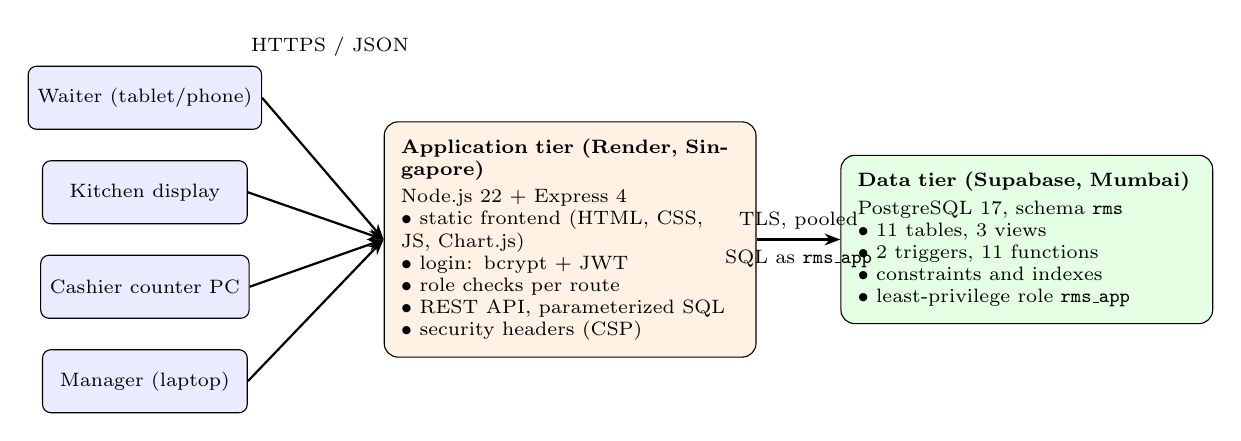
\begin{tikzpicture}
  \node[dev] (w) at (0,1.8) {Waiter (tablet/phone)};
  \node[dev] (k) at (0,0.6) {Kitchen display};
  \node[dev] (c) at (0,-0.6) {Cashier counter PC};
  \node[dev] (m) at (0,-1.8) {Manager (laptop)};
  \node[tier=orange!10] (app) at (5.4,0) {\textbf{Application tier (Render, Singapore)}\\[2pt]
     Node.js 22 + Express 4\\
     $\bullet$ static frontend (HTML, CSS, JS, Chart.js)\\
     $\bullet$ login: bcrypt + JWT\\
     $\bullet$ role checks per route\\
     $\bullet$ REST API, parameterized SQL\\
     $\bullet$ security headers (CSP)};
  \node[tier=green!10] (db) at (11.2,0) {\textbf{Data tier (Supabase, Mumbai)}\\[2pt]
     PostgreSQL 17, schema \texttt{rms}\\
     $\bullet$ 11 tables, 3 views\\
     $\bullet$ 2 triggers, 11 functions\\
     $\bullet$ constraints and indexes\\
     $\bullet$ least-privilege role \texttt{rms\_app}};
  \foreach \x in {w,k,c,m} \draw[flow] (\x.east) -- (app.west);
  \draw[flow] (app.east) -- node[lbl,above]{TLS, pooled} node[lbl,below]{SQL as \texttt{rms\_app}} (db.west);
  \node[lbl] at (2.35,2.45) {HTTPS / JSON};
\end{tikzpicture}
\caption{Three-tier architecture of the deployed system}
\label{fig:arch}
\end{figure}

\begin{table}[H]
    \centering
    \caption{Technology stack}
    \small
    \setstretch{1.15}
    \begin{tabularx}{\textwidth}{|l|Y|Y|}
        \hline
        \textbf{Layer} & \textbf{Technology} & \textbf{Purpose} \\ \hline
        Database & PostgreSQL 17 (Supabase) & Tables, constraints, triggers, PL/pgSQL functions, views (895 lines of SQL) \\ \hline
        Backend & Node.js 22, Express 4, \texttt{pg}, \texttt{bcryptjs}, \texttt{jsonwebtoken} & REST API, authentication, authorization (592 lines) \\ \hline
        Frontend & HTML5, CSS3, JavaScript (ES modules), Chart.js 4 & Single-page app for all four roles, no build step (1,379 lines) \\ \hline
        Hosting & Render (web service), Supabase (database) & Live deployment with automatic redeploy on every Git push \\ \hline
        Testing & Playwright (Chromium), curl, smoke-test script & End-to-end UI walk-through, API rule tests, post-deploy checks \\ \hline
    \end{tabularx}
\end{table}

\subsection{Database Design}
\subsubsection{Relational Schema}
Figure~\ref{fig:schema} shows the eleven relations. Arrows point from a foreign key to the referenced table.

\begin{figure}[H]
\centering
\resizebox{\textwidth}{!}{%
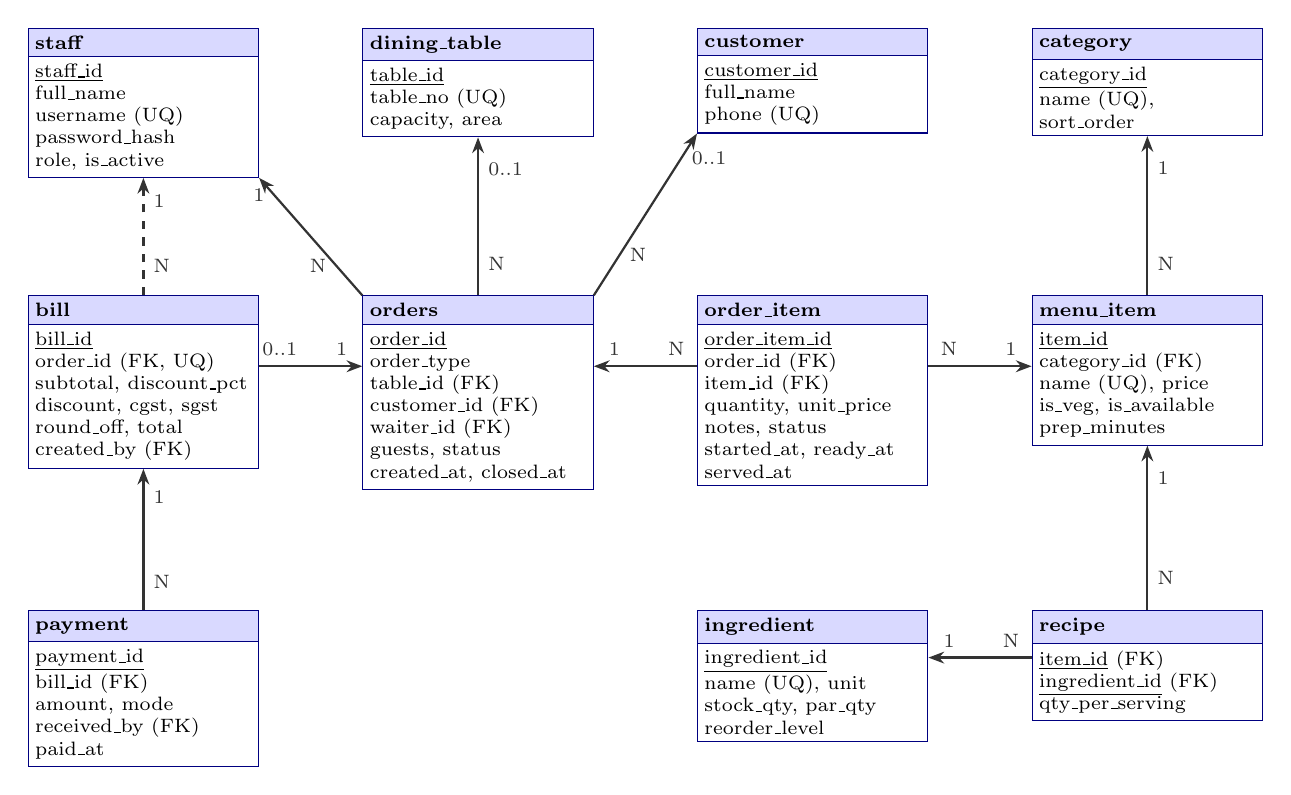
\begin{tikzpicture}
  % Row A
  \node[tbl] (staff) at (0,0) {\textbf{staff}\nodepart{two}\underline{staff\_id}\\full\_name\\username (UQ)\\password\_hash\\role, is\_active};
  \node[tbl] (dt) at (4.25,0) {\textbf{dining\_table}\nodepart{two}\underline{table\_id}\\table\_no (UQ)\\capacity, area};
  \node[tbl] (cust) at (8.5,0) {\textbf{customer}\nodepart{two}\underline{customer\_id}\\full\_name\\phone (UQ)};
  \node[tbl] (cat) at (12.75,0) {\textbf{category}\nodepart{two}\underline{category\_id}\\name (UQ), sort\_order};
  % Row B
  \node[tbl] (bill) at (0,-3.4) {\textbf{bill}\nodepart{two}\underline{bill\_id}\\order\_id (FK, UQ)\\subtotal, discount\_pct\\discount, cgst, sgst\\round\_off, total\\created\_by (FK)};
  \node[tbl] (ord) at (4.25,-3.4) {\textbf{orders}\nodepart{two}\underline{order\_id}\\order\_type\\table\_id (FK)\\customer\_id (FK)\\waiter\_id (FK)\\guests, status\\created\_at, closed\_at};
  \node[tbl] (oi) at (8.5,-3.4) {\textbf{order\_item}\nodepart{two}\underline{order\_item\_id}\\order\_id (FK)\\item\_id (FK)\\quantity, unit\_price\\notes, status\\started\_at, ready\_at\\served\_at};
  \node[tbl] (mi) at (12.75,-3.4) {\textbf{menu\_item}\nodepart{two}\underline{item\_id}\\category\_id (FK)\\name (UQ), price\\is\_veg, is\_available\\prep\_minutes};
  % Row C
  \node[tbl] (pay) at (0,-7.4) {\textbf{payment}\nodepart{two}\underline{payment\_id}\\bill\_id (FK)\\amount, mode\\received\_by (FK)\\paid\_at};
  \node[tbl] (ing) at (8.5,-7.4) {\textbf{ingredient}\nodepart{two}\underline{ingredient\_id}\\name (UQ), unit\\stock\_qty, par\_qty\\reorder\_level};
  \node[tbl] (rec) at (12.75,-7.4) {\textbf{recipe}\nodepart{two}\underline{item\_id} (FK)\\\underline{ingredient\_id} (FK)\\qty\_per\_serving};
  % relationships (child -> parent)
  \draw[fk] (ord.north) -- node[lbl,right,pos=0.2]{N} node[lbl,right,pos=0.8]{0..1} (dt.south);
  \draw[fk] (ord.north west) -- node[lbl,left,pos=0.25]{N} node[lbl,left,pos=0.85]{1} (staff.south east);
  \draw[fk] (ord.north east) -- node[lbl,right,pos=0.25]{N} node[lbl,right,pos=0.85]{0..1} (cust.south west);
  \draw[fk] (oi.west |- 0,-4.3) -- node[lbl,above,pos=0.2]{N} node[lbl,above,pos=0.8]{1} (ord.east |- 0,-4.3);
  \draw[fk] (oi.east |- 0,-4.3) -- node[lbl,above,pos=0.2]{N} node[lbl,above,pos=0.8]{1} (mi.west |- 0,-4.3);
  \draw[fk] (mi.north) -- node[lbl,right,pos=0.2]{N} node[lbl,right,pos=0.8]{1} (cat.south);
  \draw[fk] (bill.east |- 0,-4.3) -- node[lbl,above,pos=0.2]{0..1} node[lbl,above,pos=0.8]{1} (ord.west |- 0,-4.3);
  \draw[fk, dashed] (bill.north) -- node[lbl,right,pos=0.25]{N} node[lbl,right,pos=0.8]{1} (staff.south);
  \draw[fk] (pay.north) -- node[lbl,right,pos=0.2]{N} node[lbl,right,pos=0.8]{1} (bill.south);
  \draw[fk] (rec.north) -- node[lbl,right,pos=0.2]{N} node[lbl,right,pos=0.8]{1} (mi.south);
  \draw[fk] (rec.west |- 0,-8.0) -- node[lbl,above,pos=0.2]{N} node[lbl,above,pos=0.8]{1} (ing.east |- 0,-8.0);
\end{tikzpicture}}
\caption{Relational schema of the RMS (PK underlined, FK = foreign key, UQ = unique)}
\label{fig:schema}
\end{figure}

\subsubsection{Normalization and Design Decisions}
Every relation is in BCNF. Each non-key attribute depends only on the key of its own table, and the many-to-many link between dishes and ingredients is resolved by \texttt{recipe}. Four decisions deserve explanation:
\begin{enumerate}
    \item \textbf{Price snapshot.} \texttt{order\_item.unit\_price} looks like a copy of \texttt{menu\_item.price}, but it is not redundant. It records the price \emph{at the moment of sale}, so a later price change never alters an old bill.
    \item \textbf{Table status is derived, not stored.} The view \texttt{v\_table\_status} computes \texttt{FREE}, \texttt{OCCUPIED}, \texttt{FOOD\_READY} or \texttt{BILLING} from the table's open order. A stored status column could fall out of step with the orders; a derived one cannot.
    \item \textbf{Order status is controlled redundancy.} \texttt{orders.status} could be computed from the dish statuses, but it is stored for fast filtering. It is kept correct by a trigger, so no program can set it to a contradictory value.
    \item \textbf{One open order per table} is enforced by a partial unique index:
\end{enumerate}
\begin{lstlisting}[caption={Key constraints from \texttt{01\_schema.sql}}]
CREATE TABLE orders (
    order_id    SERIAL      PRIMARY KEY,
    order_type  VARCHAR(8)  NOT NULL CHECK (order_type IN ('DINE_IN','TAKEAWAY')),
    table_id    INT         REFERENCES dining_table,
    customer_id INT         REFERENCES customer,
    waiter_id   INT         NOT NULL REFERENCES staff,
    guests      SMALLINT    CHECK (guests BETWEEN 1 AND 20),
    status      VARCHAR(10) NOT NULL DEFAULT 'PLACED'
                CHECK (status IN ('PLACED','PREPARING','READY','SERVED','BILLED','PAID','CANCELLED')),
    created_at  TIMESTAMPTZ NOT NULL DEFAULT now(),
    closed_at   TIMESTAMPTZ,
    CHECK ((order_type = 'DINE_IN') = (table_id IS NOT NULL))     -- dine-in <=> has a table
);
-- A table can have only ONE open order at a time
CREATE UNIQUE INDEX uq_open_order_per_table ON orders (table_id)
    WHERE status NOT IN ('PAID','CANCELLED');

CREATE TABLE ingredient (
    ingredient_id SERIAL        PRIMARY KEY,
    name          VARCHAR(40)   NOT NULL UNIQUE,
    unit          VARCHAR(4)    NOT NULL CHECK (unit IN ('kg','l','pcs')),
    stock_qty     NUMERIC(10,3) NOT NULL CHECK (stock_qty >= 0),   -- never negative
    reorder_level NUMERIC(10,3) NOT NULL DEFAULT 0,
    par_qty       NUMERIC(10,3) NOT NULL DEFAULT 0,
    cost_per_unit NUMERIC(8,2)  NOT NULL DEFAULT 0
);
\end{lstlisting}

\subsection{Business Rules Inside the Database}
\subsubsection{Order Life-Cycle}
Each dish of an order moves through the kitchen independently, and the order status follows from its dishes (Figure~\ref{fig:life}).

\begin{figure}[H]
\centering
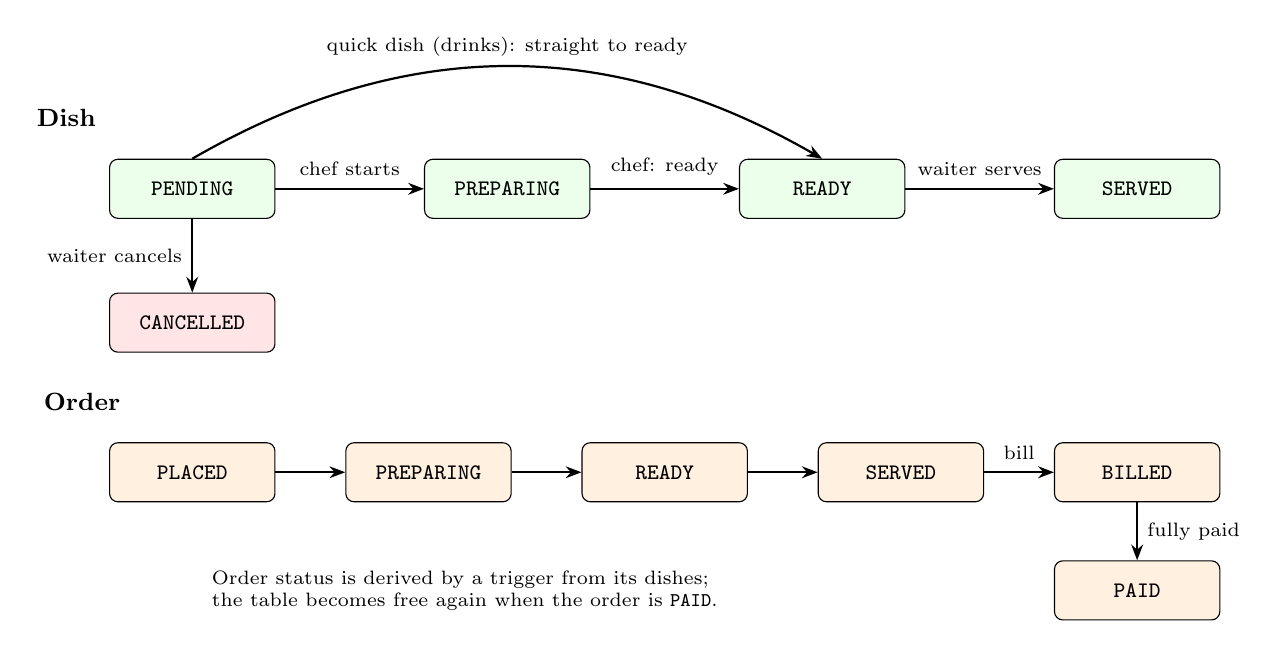
\begin{tikzpicture}
  \node[st] (p) at (0,0) {PENDING};
  \node[st] (pr) at (4,0) {PREPARING};
  \node[st] (r) at (8,0) {READY};
  \node[st] (s) at (12,0) {SERVED};
  \node[st, fill=red!10] (x) at (0,-1.7) {CANCELLED};
  \draw[tr] (p) -- node[lbl,above=1pt]{chef starts} (pr);
  \draw[tr] (pr) -- node[lbl,above=1pt]{chef: ready} (r);
  \draw[tr] (r) -- node[lbl,above=1pt]{waiter serves} (s);
  \draw[tr] (p) -- node[lbl,left]{waiter cancels} (x);
  \draw[tr] (p.north) to[out=30,in=150] node[lbl,above]{quick dish (drinks): straight to ready} (r.north);
  \node[font=\small\bfseries] at (-1.6,0.9) {Dish};
  \node[st, fill=orange!12] (op) at (0,-3.6) {PLACED};
  \node[st, fill=orange!12] (opr) at (3,-3.6) {PREPARING};
  \node[st, fill=orange!12] (ord) at (6,-3.6) {READY};
  \node[st, fill=orange!12] (os) at (9,-3.6) {SERVED};
  \node[st, fill=orange!12] (ob) at (12,-3.6) {BILLED};
  \node[st, fill=orange!12] (opd) at (12,-5.1) {PAID};
  \draw[tr] (op) -- (opr); \draw[tr] (opr) -- (ord); \draw[tr] (ord) -- (os);
  \draw[tr] (os) -- node[lbl,above=1pt]{bill} (ob);
  \draw[tr] (ob) -- node[lbl,right]{fully paid} (opd);
  \node[font=\small\bfseries] at (-1.4,-2.7) {Order};
  \node[lbl, text width=7.5cm, align=left] at (4,-5.1) {Order status is derived by a trigger from its dishes;\\the table becomes free again when the order is \texttt{PAID}.};
\end{tikzpicture}
\caption{State machines enforced by the database}
\label{fig:life}
\end{figure}

\subsubsection{Triggers}
Two row-level triggers on \texttt{order\_item} carry most of the logic. The \texttt{BEFORE} trigger rejects illegal moves and records timestamps. The \texttt{AFTER} trigger deducts (or returns) ingredient stock and recalculates the order status.

\begin{lstlisting}[caption={State-machine trigger (from \texttt{02\_logic.sql})}]
CREATE FUNCTION trg_order_item_rules() RETURNS TRIGGER
LANGUAGE plpgsql AS $$
DECLARE
    v_order_status VARCHAR;
BEGIN
    IF is_seeding() THEN RETURN NEW; END IF;          -- demo-history loader only

    SELECT status INTO v_order_status FROM orders WHERE order_id = NEW.order_id;
    IF v_order_status IN ('BILLED','PAID','CANCELLED') THEN
        RAISE EXCEPTION 'Order % is % and can no longer be changed', NEW.order_id, v_order_status;
    END IF;
    IF TG_OP = 'INSERT' THEN
        NEW.status := 'PENDING';
        RETURN NEW;
    END IF;
    IF NEW.status = OLD.status THEN RETURN NEW; END IF;
    IF NOT ((OLD.status = 'PENDING'   AND NEW.status IN ('PREPARING','READY','CANCELLED'))
         OR (OLD.status = 'PREPARING' AND NEW.status = 'READY')
         OR (OLD.status = 'READY'     AND NEW.status = 'SERVED')) THEN
        RAISE EXCEPTION 'Item cannot move from % to %', OLD.status, NEW.status;
    END IF;
    IF NEW.status IN ('PREPARING','READY') AND NEW.started_at IS NULL THEN
        NEW.started_at := now();
    END IF;
    IF NEW.status = 'READY'  THEN NEW.ready_at  := now(); END IF;
    IF NEW.status = 'SERVED' THEN NEW.served_at := now(); END IF;
    RETURN NEW;
END $$;

CREATE TRIGGER order_item_rules
    BEFORE INSERT OR UPDATE OF status ON order_item
    FOR EACH ROW EXECUTE FUNCTION trg_order_item_rules();
\end{lstlisting}

\begin{lstlisting}[caption={Stock-deduction trigger (abridged)}]
CREATE FUNCTION trg_order_item_effects() RETURNS TRIGGER
LANGUAGE plpgsql AS $$
DECLARE
    v_short RECORD;
BEGIN
    IF is_seeding() THEN RETURN NULL; END IF;
    IF TG_OP = 'INSERT' THEN
        -- lock the ingredient rows in a fixed order (prevents deadlocks)
        PERFORM 1 FROM ingredient
         WHERE ingredient_id IN (SELECT ingredient_id FROM recipe WHERE item_id = NEW.item_id)
         ORDER BY ingredient_id FOR UPDATE;
        SELECT m.name AS dish, i.name AS ingredient, i.unit, i.stock_qty,
               r.qty_per_serving * NEW.quantity AS needed INTO v_short
          FROM recipe r JOIN ingredient i ON i.ingredient_id = r.ingredient_id
                        JOIN menu_item  m ON m.item_id = r.item_id
         WHERE r.item_id = NEW.item_id AND i.stock_qty < r.qty_per_serving * NEW.quantity
         LIMIT 1;
        IF FOUND THEN
            RAISE EXCEPTION 'Not enough % for % x % (need % %, only % % left)',
                v_short.ingredient, NEW.quantity, v_short.dish,
                v_short.needed, v_short.unit, v_short.stock_qty, v_short.unit;
        END IF;
        UPDATE ingredient i SET stock_qty = i.stock_qty - r.qty_per_serving * NEW.quantity
          FROM recipe r WHERE r.item_id = NEW.item_id AND r.ingredient_id = i.ingredient_id;
    ELSIF NEW.status = 'CANCELLED' AND OLD.status = 'PENDING' THEN
        UPDATE ingredient i SET stock_qty = i.stock_qty + r.qty_per_serving * NEW.quantity
          FROM recipe r WHERE r.item_id = NEW.item_id AND r.ingredient_id = i.ingredient_id;
    END IF;
    PERFORM fn_refresh_order_status(NEW.order_id);    -- derive the order status
    RETURN NULL;
END $$;
\end{lstlisting}

\subsubsection{Stored Functions}
The API never writes order rows directly. It calls one function per business action, and each call runs as a single atomic transaction:

\begin{table}[H]
    \centering
    \caption{Business functions}
    \small
    \setstretch{1.15}
    \begin{tabularx}{\textwidth}{|l|Y|}
        \hline
        \textbf{Function} & \textbf{What it guarantees} \\ \hline
        \texttt{fn\_place\_order} & Valid table, table not already occupied, guests $\le$ capacity, at least one dish; serialised per table with an advisory lock; creates or reuses the takeaway customer by phone. \\ \hline
        \texttt{fn\_add\_items} & Order still open; each dish exists and is available; quantity 1--50; price snapshot taken. \\ \hline
        \texttt{fn\_cancel\_order} & Cancels only if the kitchen has not started any dish; stock is returned by the trigger. \\ \hline
        \texttt{fn\_generate\_bill} & Only when every dish is served; discount 0--50\%; GST and rounding computed in one place. \\ \hline
        \texttt{fn\_record\_payment} & No over-payment; supports split payments (cash + UPI); closes the order and frees the table at zero balance. \\ \hline
    \end{tabularx}
\end{table}

\begin{lstlisting}[caption={Placing an order (abridged from \texttt{fn\_place\_order})}]
IF p_type = 'DINE_IN' THEN
    -- serialise concurrent orders for the same table
    PERFORM pg_advisory_xact_lock(hashtext('rms.table'), COALESCE(p_table, 0));
    SELECT capacity INTO v_capacity FROM dining_table WHERE table_id = p_table;
    IF NOT FOUND THEN RAISE EXCEPTION 'Choose a valid table'; END IF;
    IF EXISTS (SELECT 1 FROM orders WHERE table_id = p_table
                  AND status NOT IN ('PAID','CANCELLED')) THEN
        RAISE EXCEPTION 'This table already has an open order';
    END IF;
    IF p_guests IS NULL OR p_guests < 1 OR p_guests > v_capacity THEN
        RAISE EXCEPTION 'This table seats 1 to % guests', v_capacity;
    END IF;
END IF;
INSERT INTO orders (order_type, table_id, customer_id, waiter_id, guests)
VALUES (p_type, p_table, v_customer, p_waiter, p_guests) RETURNING order_id INTO v_order;
PERFORM fn_add_items(v_order, p_items);   -- inserts dishes; triggers deduct stock
RETURN v_order;
\end{lstlisting}

\subsubsection{Mathematical Model}
\textbf{Stock deduction.} When $n$ plates of dish $m$ are ordered, every ingredient $i$ in its recipe is reduced by
$$s_i \leftarrow s_i - n \cdot q_{m,i}, \qquad \text{subject to } s_i \ge 0,$$
where $q_{m,i}$ is the quantity per serving. The \texttt{CHECK (stock\_qty >= 0)} constraint makes the condition absolute, even for simultaneous orders.

\textbf{Plates still possible.} The view \texttt{v\_menu\_stock} tells the waiter how many more plates of a dish the current stock allows:
$$\text{servings}(m) = \min_{i \in \text{recipe}(m)} \left\lfloor \frac{s_i}{q_{m,i}} \right\rfloor$$

\textbf{GST bill.} Restaurant service in India is taxed at 5\% GST (CGST 2.5\% + SGST 2.5\%). With subtotal $S = \sum_j q_j p_j$ and discount rate $d$:
\begin{align*}
D &= \text{round}_2\!\left(S \cdot \tfrac{d}{100}\right), \qquad T = S - D,\\
\text{CGST} &= \text{SGST} = \text{round}_2(0.025\,T), \qquad
\text{Total} = \text{round}_0\big(T + \text{CGST} + \text{SGST}\big).
\end{align*}
\textit{Worked example (live test, order of 2 Chicken Biryani, 1 Butter Chicken, 3 Butter Naan, 1 Irani Chai):} $S = 640 + 340 + 180 + 40 = 1200$; with $d = 10$, $D = 120$, $T = 1080$, CGST $=$ SGST $= 27.00$, Total $=$ Rs.\,1,134. The receipt in Figure~\ref{fig:billing} shows exactly these figures.

\subsection{Analytical Queries for the Dashboard}
The manager's dashboard is built from SQL aggregate and window queries. Two examples:

\begin{lstlisting}[caption={Top dishes (window function) and kitchen speed}]
-- Top dishes in the selected period
SELECT RANK() OVER (ORDER BY SUM(oi.quantity) DESC) AS rnk, m.name,
       SUM(oi.quantity) AS qty, SUM(oi.quantity * oi.unit_price) AS revenue
  FROM order_item oi
  JOIN orders o    ON o.order_id = oi.order_id
  JOIN menu_item m ON m.item_id  = oi.item_id
 WHERE o.status = 'PAID' AND o.created_at >= $1 AND oi.status <> 'CANCELLED'
 GROUP BY m.item_id, m.name
 ORDER BY rnk LIMIT 8;

-- Average preparation time and order-to-table time per dish
SELECT m.name, m.prep_minutes AS target,
       ROUND(AVG(EXTRACT(EPOCH FROM (oi.ready_at  - oi.started_at)) / 60)::numeric, 1) AS avg_prep,
       ROUND(AVG(EXTRACT(EPOCH FROM (oi.served_at - oi.created_at)) / 60)::numeric, 1) AS avg_to_table
  FROM order_item oi
  JOIN orders o    ON o.order_id = oi.order_id
  JOIN menu_item m ON m.item_id  = oi.item_id
 WHERE o.created_at >= $1 AND oi.served_at IS NOT NULL
 GROUP BY m.item_id, m.name, m.prep_minutes
 ORDER BY avg_to_table DESC LIMIT 6;
\end{lstlisting}

Results on the live database (30 days of generated demo history, 1,026 orders):
\begin{table}[H]
    \centering
    \caption{Live query results (last 30 days)}
    \footnotesize
    \begin{minipage}[t]{0.48\textwidth}\centering
    \begin{tabular}{|c|l|r|r|}
        \hline
        \textbf{\#} & \textbf{Dish} & \textbf{Plates} & \textbf{Rs.} \\ \hline
        1 & Butter Naan & 686 & 41,160 \\ \hline
        2 & Hyd. Chicken Biryani & 413 & 1,32,160 \\ \hline
        3 & Tandoori Roti & 296 & 10,360 \\ \hline
        4 & Irani Chai & 292 & 11,680 \\ \hline
        5 & Butter Chicken & 226 & 76,840 \\ \hline
    \end{tabular}
    \end{minipage}\hfill
    \begin{minipage}[t]{0.48\textwidth}\centering
    \begin{tabular}{|l|r|r|r|}
        \hline
        \textbf{Dish} & \textbf{Target} & \textbf{Prep} & \textbf{To table} \\ \hline
        Mutton Biryani & 30 & 30.6 & 36.0 \\ \hline
        Chicken Biryani & 25 & 25.4 & 30.9 \\ \hline
        Butter Chicken & 20 & 20.3 & 25.8 \\ \hline
        Egg Biryani & 20 & 20.1 & 25.4 \\ \hline
    \end{tabular}\\[1mm]
    {\scriptsize (minutes)}
    \end{minipage}
\end{table}
Over the 30 days the system recorded 978 paid orders, revenue of Rs.\,7,85,748 and an average bill of Rs.\,803. Payments were 54\% UPI, 25\% cash and 20\% card, and the busiest hours were 8--9\,PM (243 orders) and 1--2\,PM (231 orders).

\subsection{Application Layer}
\subsubsection{REST API}
\begin{table}[H]
    \centering
    \caption{Main API endpoints (all except login require a JWT)}
    \footnotesize
    \setstretch{1.12}
    \begin{tabularx}{\textwidth}{|l|l|l|Y|}
        \hline
        \textbf{Method} & \textbf{Path} & \textbf{Roles} & \textbf{Database object} \\ \hline
        POST & \texttt{/api/auth/login} & public & \texttt{staff} (bcrypt check) \\ \hline
        GET & \texttt{/api/tables} & all & view \texttt{v\_table\_status} \\ \hline
        GET & \texttt{/api/menu} & all & \texttt{menu\_item} + view \texttt{v\_menu\_stock} \\ \hline
        POST & \texttt{/api/orders} & Waiter, Manager & \texttt{fn\_place\_order} \\ \hline
        POST & \texttt{/api/orders/:id/items} & Waiter, Manager & \texttt{fn\_add\_items} \\ \hline
        PATCH & \texttt{/api/order-items/:id} & Chef (cook), Waiter (serve) & \texttt{UPDATE order\_item} + triggers \\ \hline
        GET & \texttt{/api/kitchen} & Chef, Waiter, Manager & view \texttt{v\_kitchen\_queue} \\ \hline
        POST & \texttt{/api/orders/:id/bill} & Cashier, Manager & \texttt{fn\_generate\_bill} \\ \hline
        POST & \texttt{/api/bills/:id/payments} & Cashier, Manager & \texttt{fn\_record\_payment} \\ \hline
        GET/POST & \texttt{/api/inventory} & Chef (view), Manager & \texttt{ingredient} \\ \hline
        GET & \texttt{/api/reports/summary} & Manager & 10 aggregate queries \\ \hline
    \end{tabularx}
\end{table}

\begin{lstlisting}[style=js, caption={A route: the API only validates input and calls the database function}]
router.post('/orders', allow('WAITER'), wrap(async (req, res) => {
  const { order_type, table_id, guests, customer_name, phone, items } = req.body;
  const { rows } = await db.query(
    'SELECT fn_place_order($1, $2, $3, $4, $5, $6, $7::jsonb) AS order_id',
    [req.user.staff_id, order_type, int(table_id), int(guests), customer_name || null,
     phone || null, JSON.stringify(items || [])]
  );
  res.status(201).json(rows[0]);
}));
\end{lstlisting}

Errors raised by PL/pgSQL (\texttt{RAISE EXCEPTION}) reach the browser as clear messages, for example \emph{``Not enough Mutton for 20 x Mutton Dum Biryani (need 5.000 kg, only 4.000 kg left)''}.

\subsubsection{Security Measures}
\begin{itemize}
    \item Passwords are stored only as \textbf{bcrypt} hashes; a login returns a signed \textbf{JWT} valid for 12 hours, and repeated failed logins are throttled.
    \item Every route checks the user's \textbf{role}; the database itself is reached through the role \texttt{rms\_app}, which has no \texttt{DELETE} or \texttt{TRUNCATE} rights, cannot change staff accounts, and cannot edit bills or payments once created.
    \item All SQL uses \textbf{bound parameters} (\texttt{\$1, \$2, \ldots}), so SQL injection is not possible; the database connection uses TLS.
    \item The server sends a strict \textbf{Content-Security-Policy} and other security headers, and all text shown in the browser is HTML-escaped to prevent cross-site scripting.
\end{itemize}

\subsection{User Interface}
The frontend is a single-page application that adapts its menu to the logged-in role. Tables, kitchen and billing screens refresh automatically every few seconds, so all devices show the same live state.

\begin{figure}[H]
    \centering
    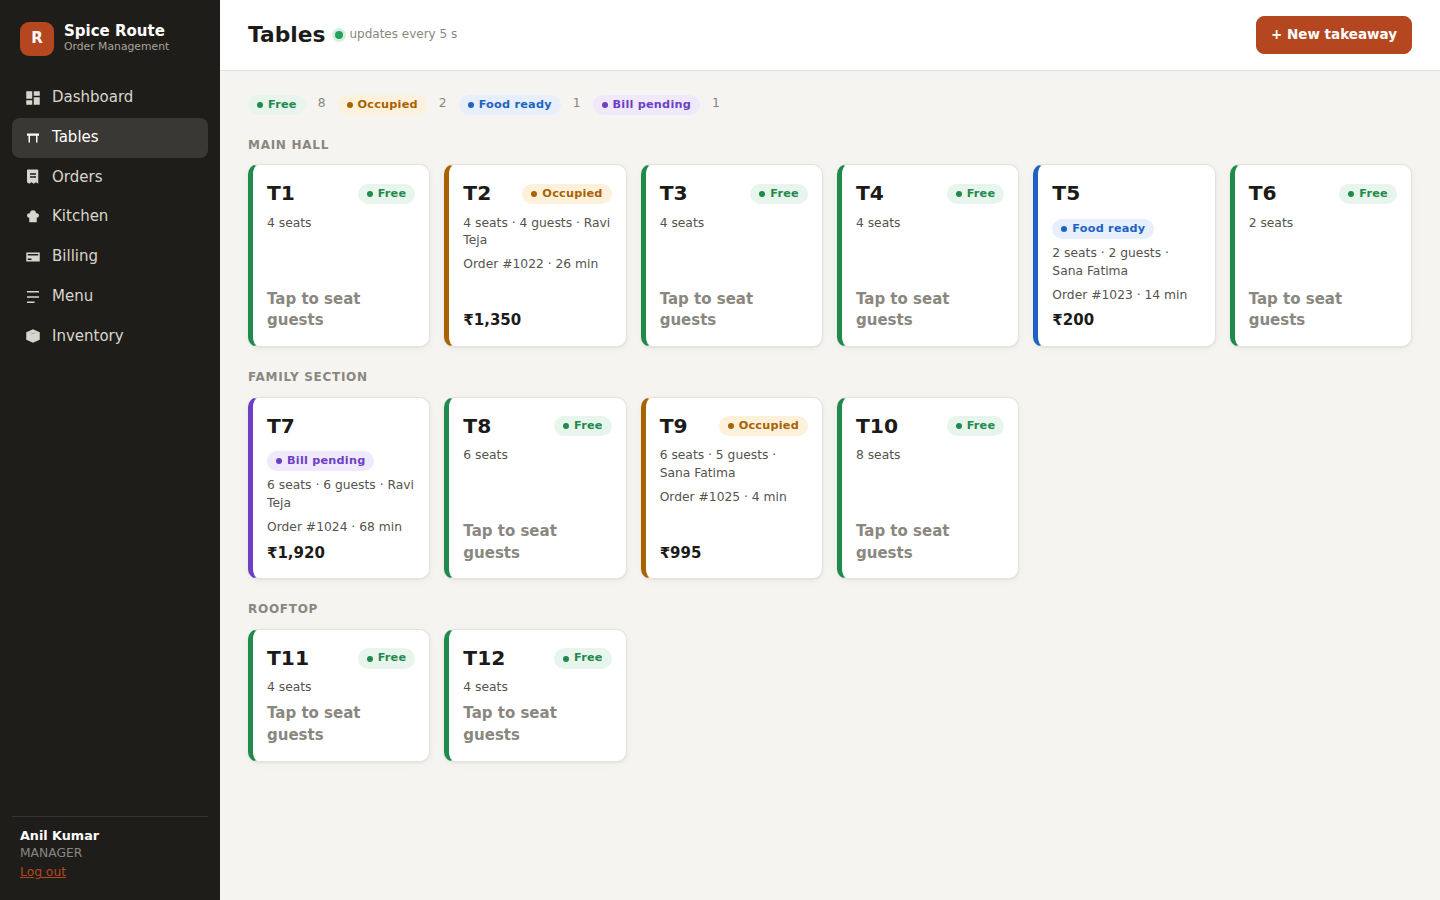
\includegraphics[width=0.95\textwidth]{03-tables.png}
    \caption{Waiter's floor plan: each table's state is derived live from its open order}
\end{figure}

\begin{figure}[H]
    \centering
    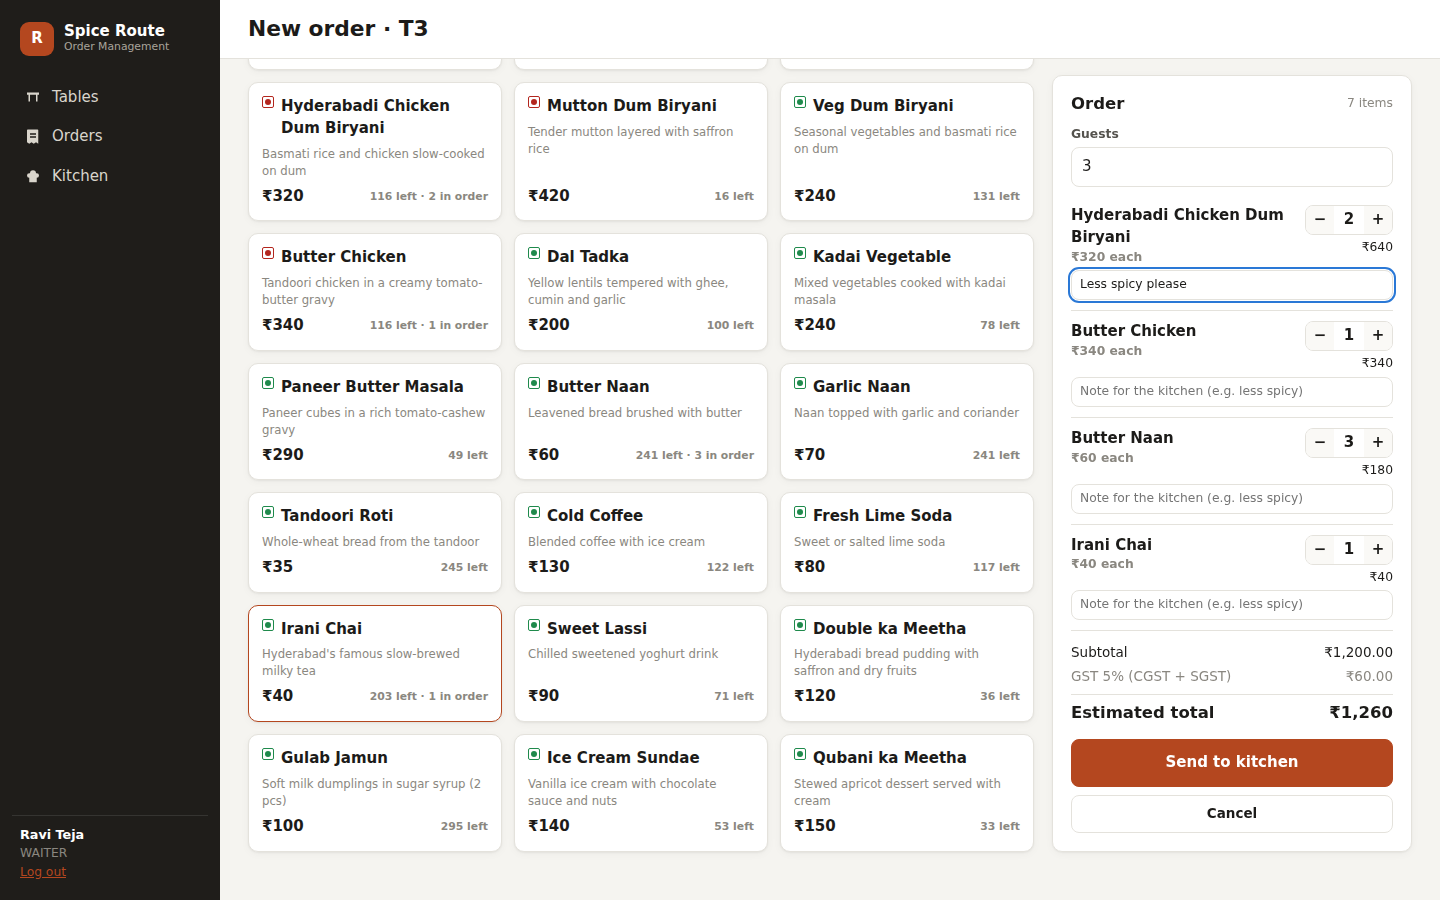
\includegraphics[width=0.95\textwidth]{04-new-order.png}
    \caption{Taking an order: menu with live ``plates left'' from stock, cart with kitchen notes and GST estimate}
\end{figure}

\begin{figure}[H]
    \centering
    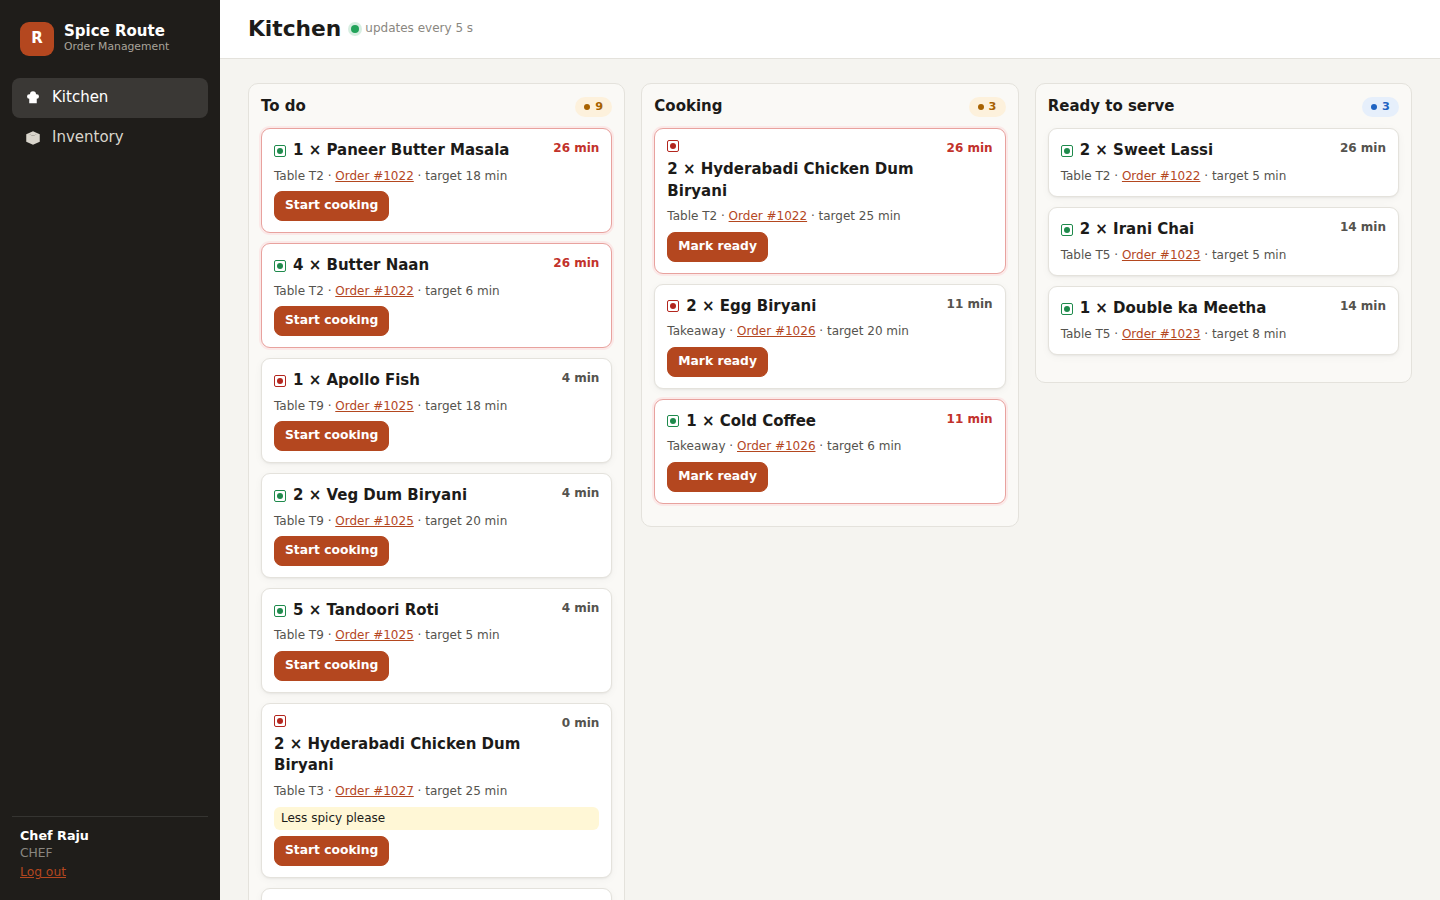
\includegraphics[width=0.95\textwidth]{06-kitchen.png}
    \caption{Kitchen display system: dishes waiting longer than their target time are highlighted in red}
\end{figure}

\begin{figure}[H]
    \centering
    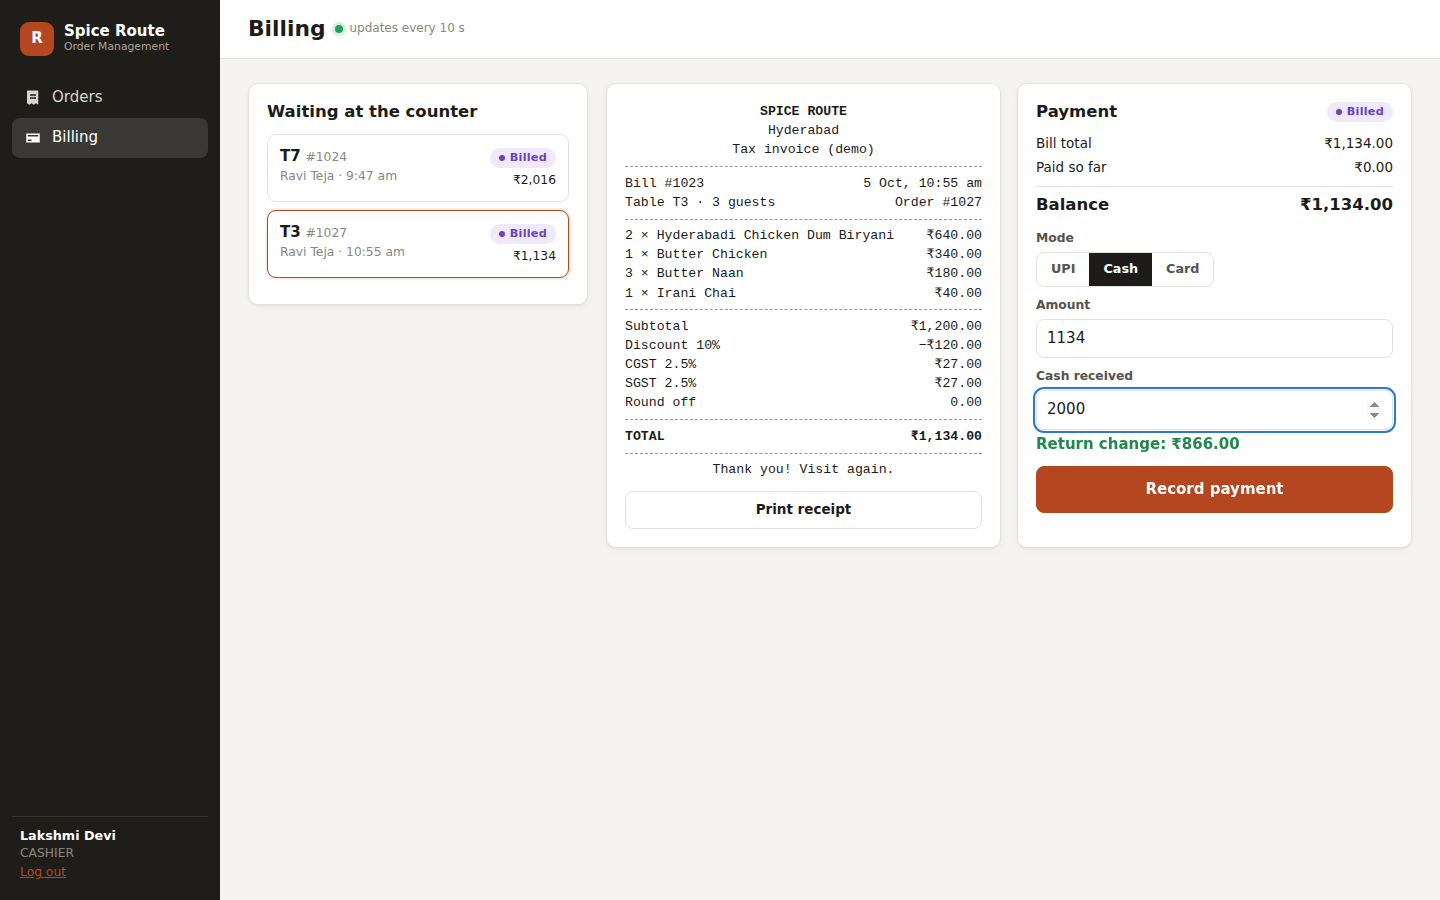
\includegraphics[width=0.95\textwidth]{08-billing-payment.png}
    \caption{Billing counter: GST receipt (10\% discount applied) and cash payment with change calculation}
    \label{fig:billing}
\end{figure}

\begin{figure}[H]
    \centering
    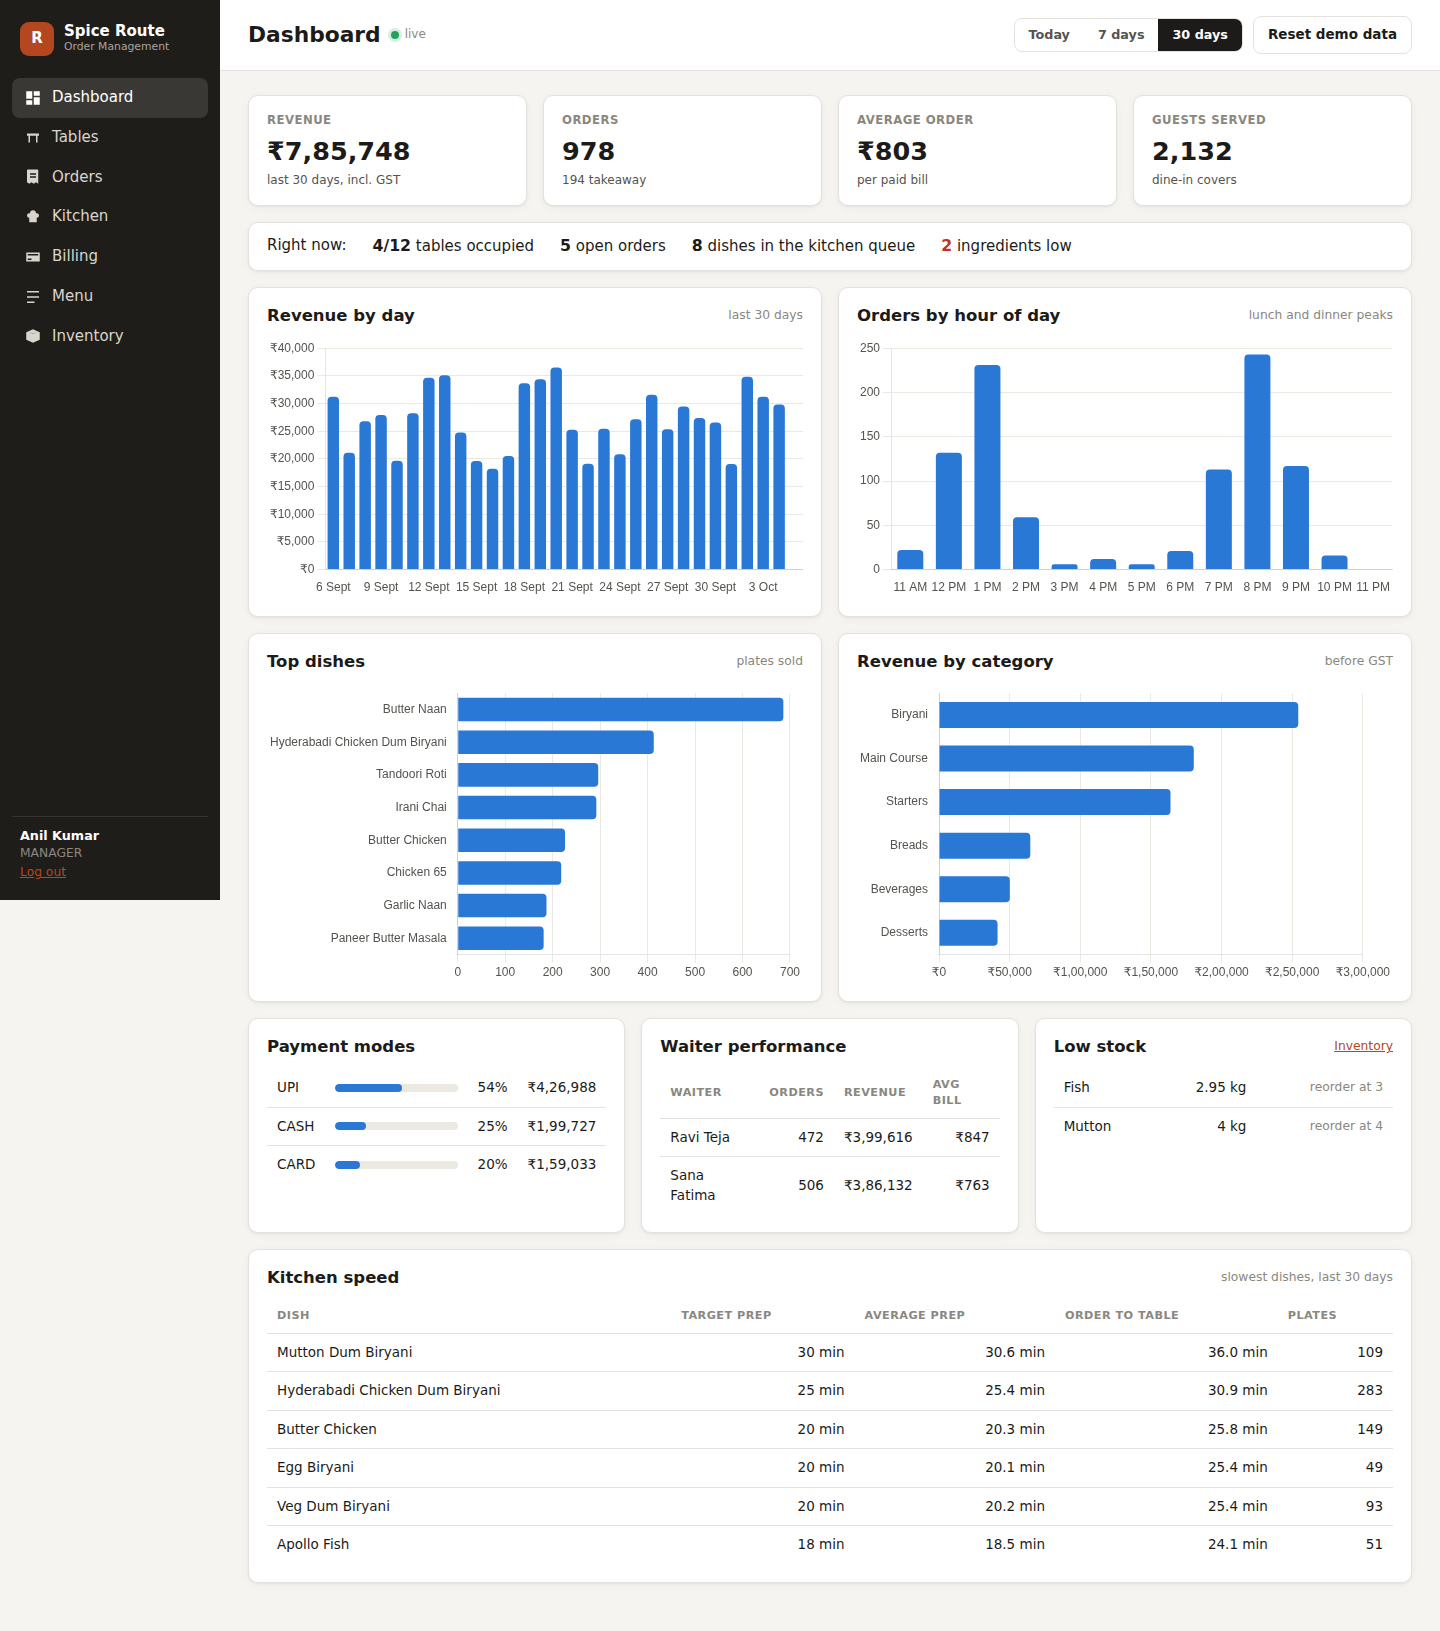
\includegraphics[width=0.88\textwidth]{02-dashboard.png}
    \caption{Manager's dashboard (last 30 days) built from the analytical queries}
\end{figure}

\begin{figure}[H]
    \centering
    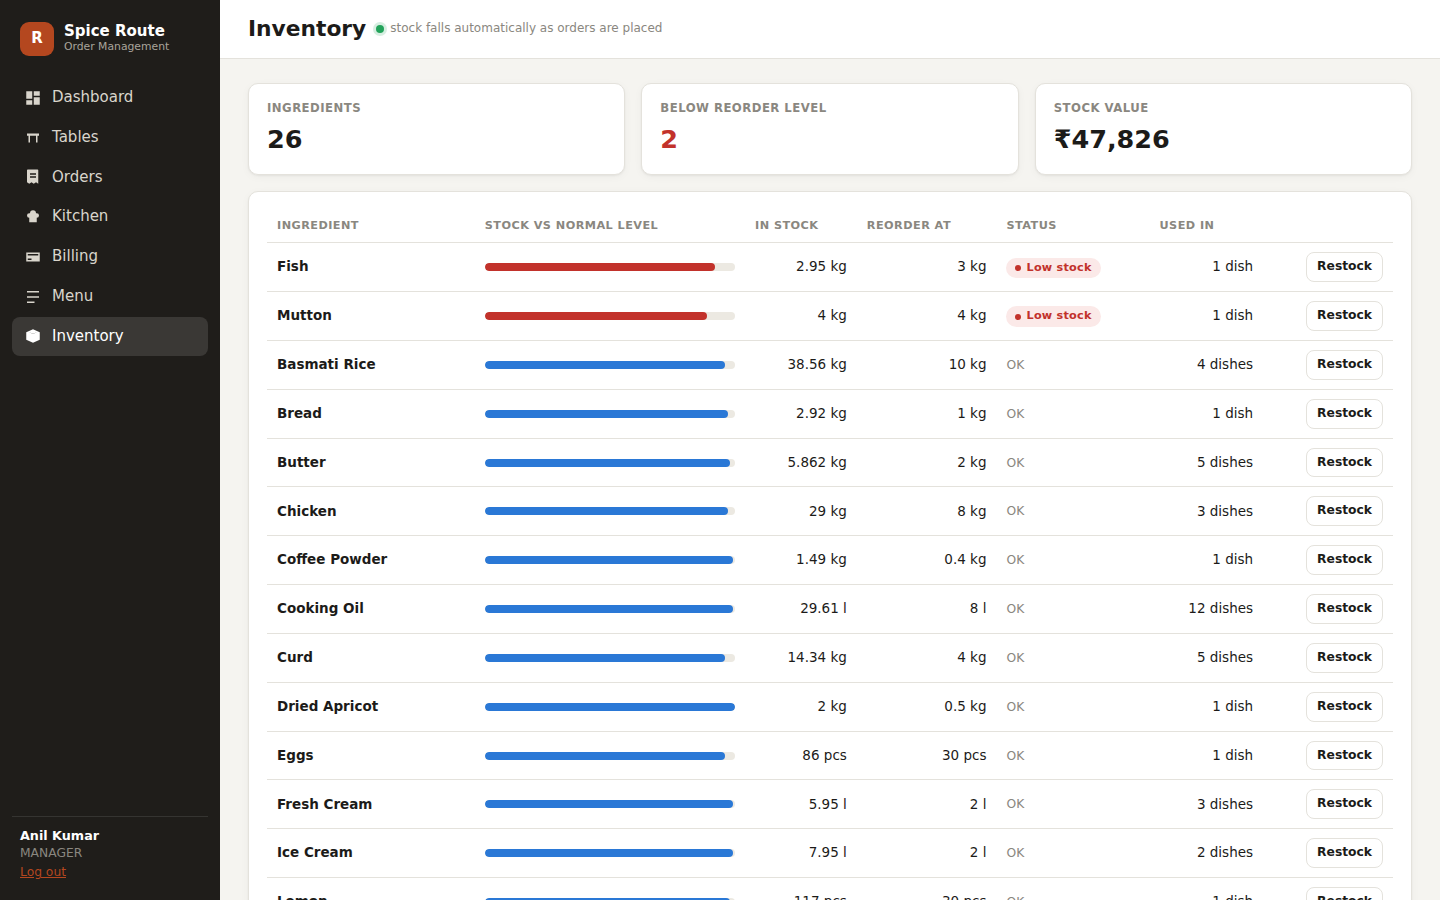
\includegraphics[width=0.95\textwidth]{10-inventory.png}
    \caption{Inventory: stock is reduced automatically by the trigger; items below reorder level are flagged}
\end{figure}

\begin{figure}[H]
    \centering
    \begin{minipage}[b]{0.62\textwidth}\centering
        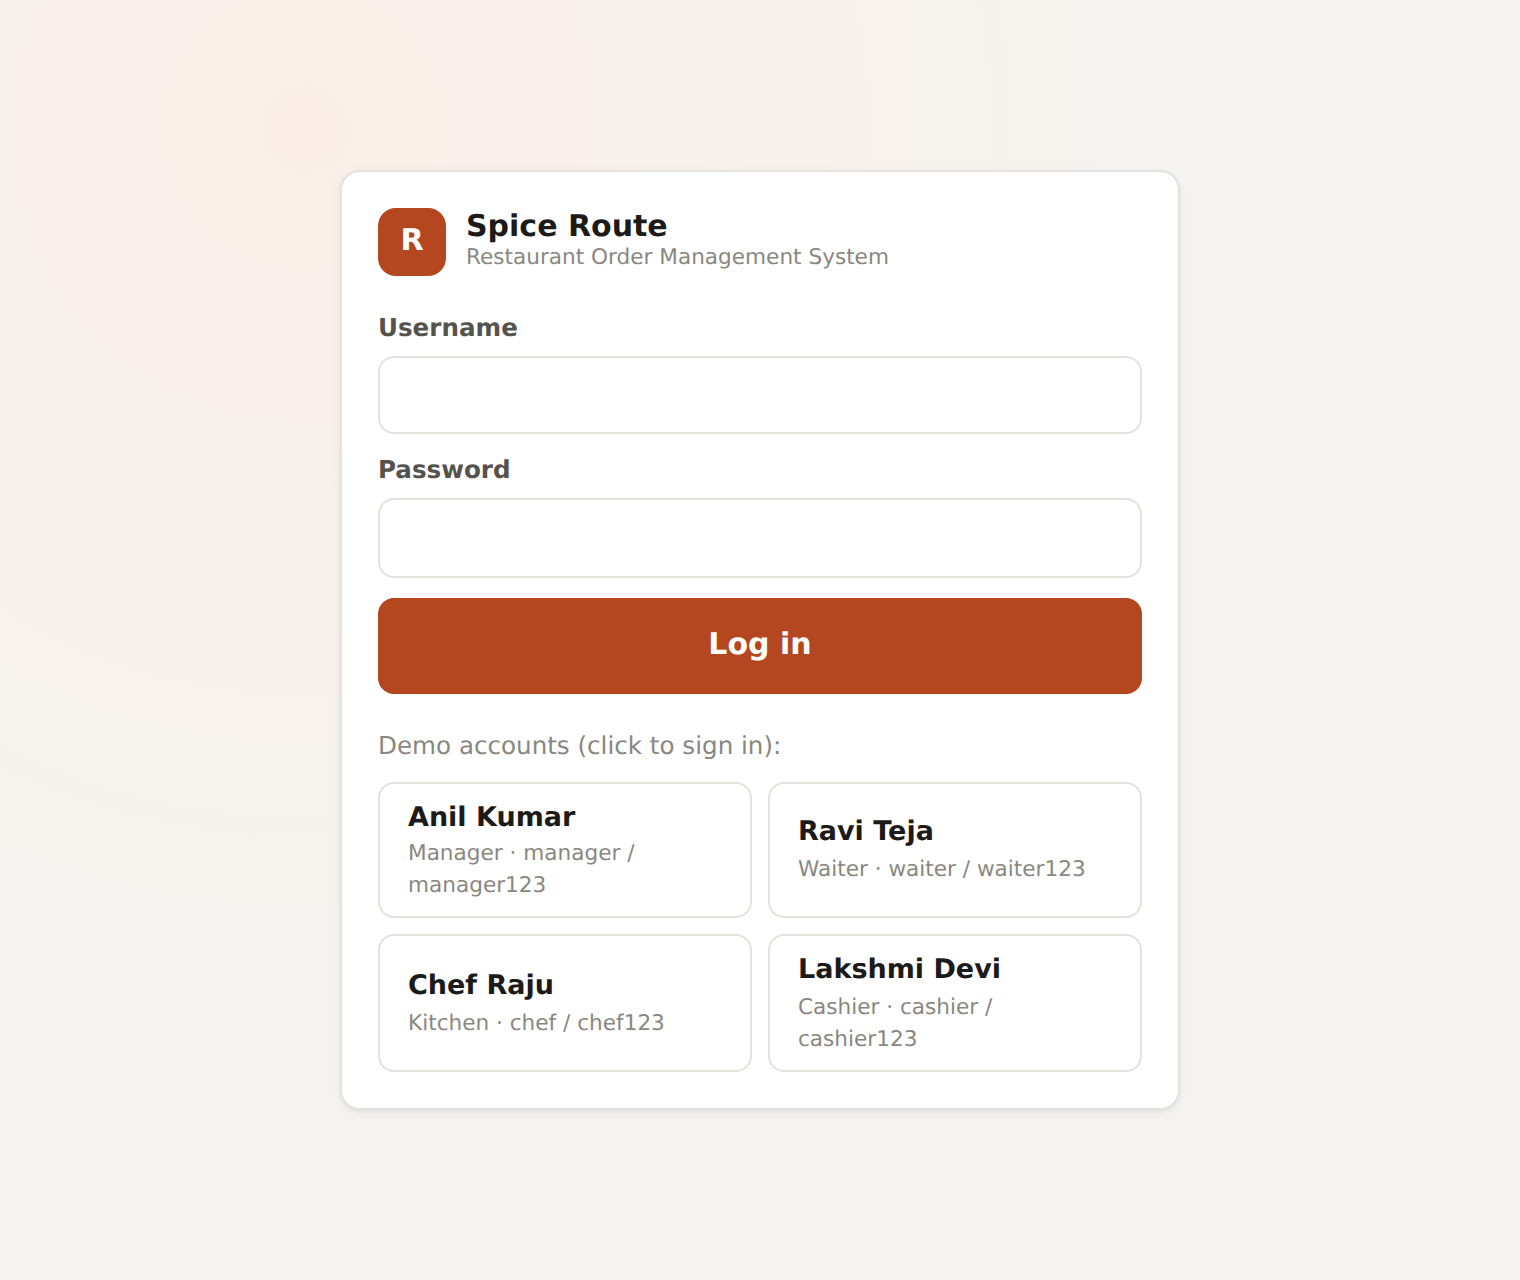
\includegraphics[width=0.7\textwidth]{01-login.png}\\[1mm]
        {\small (a) Login with demo accounts}\\[4mm]
        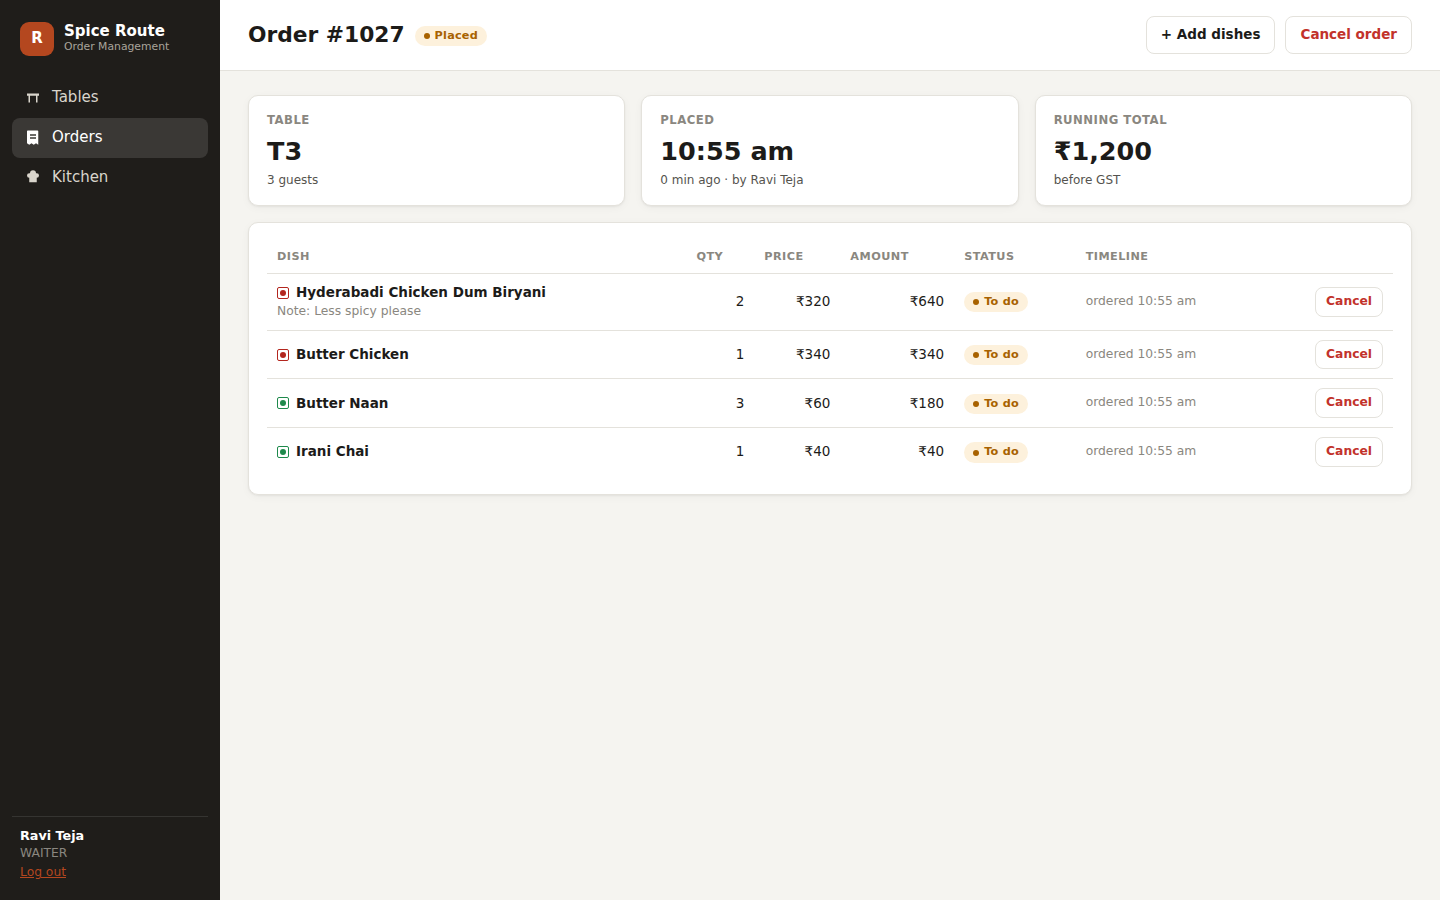
\includegraphics[width=\textwidth]{05-order-detail.png}\\[1mm]
        {\small (b) Order detail with per-dish status and timeline}
    \end{minipage}\hfill
    \begin{minipage}[b]{0.3\textwidth}\centering
        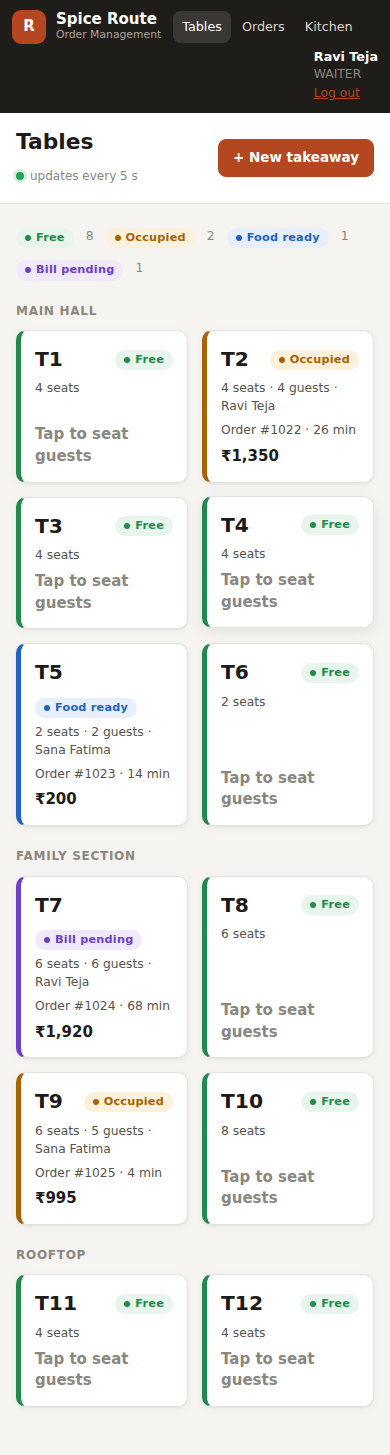
\includegraphics[width=\textwidth]{12-mobile-tables.png}\\[1mm]
        {\small (c) Phone layout}
    \end{minipage}
    \caption{Login, order detail and responsive mobile view}
\end{figure}

\subsection{Deployment}
\begin{table}[H]
    \centering
    \caption{Live deployment}
    \small
    \setstretch{1.15}
    \begin{tabularx}{\textwidth}{|l|Y|}
        \hline
        \textbf{Item} & \textbf{Details} \\ \hline
        Public URL & \url{https://spice-route-rms.onrender.com} \\ \hline
        Web service & Render, free plan, Singapore region, Node.js 22; rebuilt automatically on every push to the Git branch \\ \hline
        Database & Supabase PostgreSQL 17.11, Mumbai region (\texttt{ap-south-1}); schema \texttt{rms} created through four SQL migrations \\ \hline
        Connection & Supavisor connection pooler (session mode, TLS), user \texttt{rms\_app} \\ \hline
        Configuration & Environment variables \texttt{DATABASE\_URL}, \texttt{JWT\_SECRET}, \texttt{NODE\_VERSION}; no secrets are stored in Git \\ \hline
        Note & On the free plan the server sleeps after 15 minutes without visitors; the first request then takes up to about a minute to wake it. \\ \hline
    \end{tabularx}
\end{table}

\subsection{Testing and Validation}
The system was tested at three levels: business-rule tests against the API, an automated end-to-end walk-through in a real browser (Playwright with Chromium), and a smoke test that the deployed server runs against itself after start-up.

\begin{table}[H]
    \centering
    \caption{Test cases and observed results}
    \label{tab:tests}
    \footnotesize
    \setstretch{1.12}
    \begin{tabularx}{\textwidth}{|c|Y|Y|c|}
        \hline
        \textbf{\#} & \textbf{Test} & \textbf{Observed result} & \textbf{Pass} \\ \hline
        1 & Login with a wrong password & 401 \emph{Invalid username or password} & \checkmark \\ \hline
        2 & API call without logging in & 401 \emph{Please log in} & \checkmark \\ \hline
        3 & Waiter places a dine-in order (3 guests, 3 dishes) & Order created, dishes \texttt{PENDING}, stock reduced & \checkmark \\ \hline
        4 & Second order on an occupied table & \emph{This table already has an open order} & \checkmark \\ \hline
        5 & Order with no dishes & \emph{Add at least one item} & \checkmark \\ \hline
        6 & Chef tries to place an order & 403 \emph{This action needs one of: MANAGER, WAITER} & \checkmark \\ \hline
        7 & 20 Mutton Biryani with 4 kg mutton in stock & \emph{Not enough Mutton \ldots (need 5.000 kg, only 4.000 kg left)} & \checkmark \\ \hline
        8 & Waiter marks a dish \texttt{PREPARING} & 403 \emph{Only CHEF or MANAGER can \ldots} & \checkmark \\ \hline
        9 & Dish moved \texttt{PREPARING} $\rightarrow$ \texttt{SERVED} (skipping \texttt{READY}) & \emph{Item cannot move from PREPARING to SERVED} & \checkmark \\ \hline
        10 & All dishes marked ready & Order status became \texttt{READY} automatically (trigger) & \checkmark \\ \hline
        11 & Bill requested before all dishes served & \emph{A bill can be generated only after every item is served} & \checkmark \\ \hline
        12 & Bill for Rs.\,940 with 10\% discount & Total Rs.\,888 (CGST = SGST = 21.15, round-off $-0.30$) & \checkmark \\ \hline
        13 & Over-payment of Rs.\,900 on Rs.\,888 & \emph{Amount must be between 0.01 and 888.00} & \checkmark \\ \hline
        14 & Split payment Rs.\,500 cash + Rs.\,388 UPI & Balance 0, order \texttt{PAID}, table \texttt{FREE} & \checkmark \\ \hline
        15 & Payment on a settled bill & \emph{This bill is already settled} & \checkmark \\ \hline
        16 & Ordering a dish hidden from the menu & \emph{Ice Cream Sundae is not available right now} & \checkmark \\ \hline
        17 & Cashier opens the manager's report & 403 Forbidden & \checkmark \\ \hline
        18 & Browser walk-through: waiter $\rightarrow$ chef $\rightarrow$ waiter $\rightarrow$ cashier & Order taken, cooked, served, billed (Rs.\,1,134) and paid; 0 browser errors & \checkmark \\ \hline
        19 & Post-deploy smoke test on the live server & 18/18 checks passed (all roles, all main screens) & \checkmark \\ \hline
    \end{tabularx}
\end{table}

\subsection{Proposed Solution Strategy}
\begin{table}[H]
    \centering
    \caption{Summary of the solution}
    \vspace{2mm}
    \setstretch{1.2}
    \begin{tabular}{|l|p{10cm}|}
        \hline
        \textbf{Strategy} & \textbf{Implementation Details} \\ \hline
        Data Model & 11 normalized tables; price snapshot per order line; derived table status; partial unique index for one open order per table. \\ \hline
        Rules in the DB & State-machine and stock triggers; atomic PL/pgSQL functions for ordering, billing and payment. \\ \hline
        Concurrency & Advisory lock per table, ordered row locks on ingredients, \texttt{CHECK (stock\_qty >= 0)} as the final guarantee. \\ \hline
        Application & Express REST API, JWT + bcrypt login, role checks, parameterized SQL, least-privilege DB role. \\ \hline
        Interface & Role-aware single-page app: floor plan, order taking, kitchen display, billing, menu, inventory, dashboard. \\ \hline
        Deployment & Render web service + Supabase PostgreSQL, automatic redeploy, post-deploy smoke test. \\ \hline
    \end{tabular}
\end{table}

%% ------------------ Section 3: Program Outcome Mapping ------------------
%
%\section{Application of Program Outcomes and Sustainability Goals}
%As per the NBA SAR requirements for solving complex engineering problems incorporating sustainability, the following mapping demonstrates the technical and societal alignment of this report.
%
%\begin{table}[h!]
%    \centering
%    \renewcommand{\arraystretch}{1.4}
%    \setlength{\tabcolsep}{8pt}
%    \caption{Mapping of POs and Targeted Sustainability Goals}
%    \begin{tabular}{|c|p{8.5cm}|c|}
%        \hline
%        \textbf{PO No.} & \textbf{Relevance to Complex Engineering Problem Solving} & \textbf{Targeted SDG} \\
%        \hline
%        \textbf{PO1} & \textbf{Engineering Knowledge:} Applies normalization, triggers, transactions and web engineering to restaurant operations. & SDG 8 \\
%        \hline
%        \textbf{PO2} & \textbf{Problem Analysis:} Analyses concurrency, state consistency and billing correctness in a multi-user setting. & SDG 8 \\
%        \hline
%        \textbf{PO3} & \textbf{Design/Development:} Designs a full-stack system whose inventory tracking reduces food waste. & SDG 12 \\
%        \hline
%        \textbf{PO4} & \textbf{Investigations:} Validates the system with 19 tests and analyses sales and kitchen-speed data. & SDG 12 \\
%        \hline
%        \textbf{PO5} & \textbf{Tool Usage:} Uses PostgreSQL, Node.js, Playwright and cloud platforms (Render, Supabase). & SDG 9 \\
%        \hline
%        \textbf{PO11} & \textbf{Life-Long Learning:} Learns cloud deployment and secure web development beyond the syllabus. & SDG 9 \\
%        \hline
%    \end{tabular}
%\end{table}

% ------------------ Section 4: Sustainability ------------------

\section{Sustainability Integration}

\subsection{Reducing Food Waste and Paper}
Every dish has a recipe, so the database always knows how much of each ingredient remains. The kitchen therefore sees shortages \emph{before} a dish is promised to a customer. The dashboard's top-dish and hourly-demand data allow the manager to prepare and purchase in line with actual demand, the core lever for reducing food waste (\textbf{SDG 12}, Target 12.3). Digital kitchen tickets and on-screen bills also replace thousands of paper KOT slips each month.

\subsection{Impact on Society and Environment}
\begin{itemize}
    \item \textbf{Social and economic:} Accurate bills with correct GST build customer trust and protect the restaurant's revenue. Clear role-based screens reduce staff stress and errors, supporting decent work (\textbf{SDG 8}).
    \item \textbf{Technological inclusion:} The system runs in any browser on existing phones and PCs and is hosted on free-tier cloud services, so a small restaurant can adopt it at almost no cost (\textbf{SDG 9}).
    \item \textbf{Environmental:} The lean design (no build step, about 200\,KB of JavaScript, short polling intervals only on live screens) keeps network and server energy use low.
\end{itemize}

% ------------------ Section 5: Conclusion ------------------

\section{Conclusion and Future Directions}

\subsection{Solution Summary}
The project delivered a working, publicly deployed Restaurant Order Management System. A normalized PostgreSQL schema of eleven tables, with triggers and stored functions, guarantees correct order and dish states, automatic stock deduction, one open order per table and exact GST billing, regardless of which program changes the data. A Node.js/Express API with bcrypt, JWT and role checks connects a responsive single-page frontend for waiters, the kitchen, cashiers and the manager. All nineteen tests passed, including a browser walk-through of a complete order and a post-deployment smoke test on the live server.

\subsection{Future Scope}
Future versions can add \textbf{QR-code table ordering} by customers, \textbf{UPI payment-gateway} integration, and \textbf{WebSocket} push updates in place of polling. Other extensions are \textbf{thermal-printer} support for kitchen tickets and receipts, \textbf{multi-branch} management, a \textbf{loyalty programme} using the customer table, and \textbf{machine-learning demand forecasting} for automatic purchase suggestions.

% ------------------ Section 6: References ------------------

\begin{thebibliography}{99}
    \bibitem{silberschatz} A. Silberschatz, H. F. Korth and S. Sudarshan, \textit{Database System Concepts}, 7th Edition, McGraw-Hill Education, 2019.
    \bibitem{elmasri} R. Elmasri and S. B. Navathe, \textit{Fundamentals of Database Systems}, 7th Edition, Pearson Education, 2016.
    \bibitem{pgdocs} The PostgreSQL Global Development Group, \textit{PostgreSQL 17 Documentation}: Triggers, PL/pgSQL, Explicit Locking and Partial Indexes, \url{https://www.postgresql.org/docs/17/}.
    \bibitem{provos} N. Provos and D. Mazi\`{e}res, ``A Future-Adaptable Password Scheme,'' \textit{Proc. USENIX Annual Technical Conference}, 1999.
    \bibitem{jwt} M. Jones, J. Bradley and N. Sakimura, ``JSON Web Token (JWT),'' RFC 7519, IETF, 2015.
    \bibitem{fielding} R. T. Fielding, \textit{Architectural Styles and the Design of Network-based Software Architectures}, Ph.D. Dissertation, University of California, Irvine, 2000.
    \bibitem{owasp} OWASP Foundation, \textit{OWASP Top 10:2021} and \textit{SQL Injection Prevention Cheat Sheet}, \url{https://owasp.org}.
    \bibitem{gst} Central Board of Indirect Taxes and Customs, Notification No. 46/2017-Central Tax (Rate): GST on restaurant services, 2017.
    \bibitem{sdg} United Nations, \textit{Transforming Our World: The 2030 Agenda for Sustainable Development}, A/RES/70/1, 2015.
\end{thebibliography}

\end{document}
